\documentclass[11pt]{article}
\usepackage{amsmath, amssymb, amsthm}
\usepackage[retainorgcmds]{IEEEtrantools}

\usepackage[pdftex]{graphicx}
\usepackage{tikz}
\usepackage{circuitikz}
\usetikzlibrary{intersections}

\usepackage{fancyhdr}

%Format stuff
\pagestyle{fancy}
\headheight 35pt

%Header info
\chead{\Large \textbf{Mechanical Impedance and Transmission}}
\lhead{}
\rhead{}

\begin{document}
\section{Mechanical Impedance}
	For a traveling wave being driven by a transverse force operating at some constant phase and amplitude $F_0e^{i\omega t}$, the mechanical impedance of the wave is defined as the ratio between force and velocity:
	\begin{equation}
		Z_m = \frac{|F_T|}{|v_T|}
	\end{equation}
	
	Consider the free-body diagram for the start of the string:
	\begin{center}
	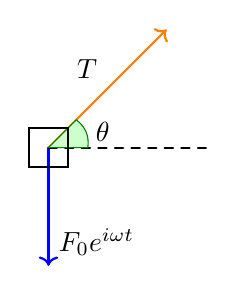
\begin{tikzpicture}
		[scale=1,line cap=round,
		%Styles
		axes/.style=,
		important line/.style={very thick},
		information text/.style={rounded corners,fill=red!10,inner sep=1ex},
		dot/.style={circle,inner sep=1pt,fill,label={#1},name=#1}			
		]
		
		%Colors
		\colorlet{anglecolor}{green!50!black}	%angle arcs/lines
		
		%The graphic
		
		\draw[->,thick,blue] (0, 0) -- (0, -1.5) node[above right,black] {$F_0e^{i\omega t}$};
		\draw[->,thick,orange] (0, 0) -- node[above left,black] {$T$} (1.5,1.5) ;
		\draw[dashed,thick] (0, 0) -- (2, 0);
		
		\coordinate (A) at (.5, .5);
		\coordinate (B) at (.5, 0);
		
		\filldraw[draw=anglecolor,fill=green!20] (0, 0) -- ($(0, 0)!5mm!(A)$) to[bend left] node[black,right] {$\theta$} (B) --cycle;
		\draw[thick] (-.25, .25) rectangle (.25, -.25);
	\end{tikzpicture}
	\end{center}
	The force is responsible for maintaining the tension in the string (otherwise there can be no traveling wave), so
	\begin{equation}
		F_0e^{i\omega t} = -T\sin\theta \approx -T \tan \theta = -T \left(\frac{\partial y}{\partial x}\right)
	\end{equation}
	At $x = 0$, this gives
	\begin{equation}
		y(x, t) = \frac{F_0v_0}{i\omega T}e^{-i(kx - \omega t)}
	\end{equation}
	
	Taking the ratio of transverse force to transverse velocity gives
	\begin{equation}
		Z_m = \frac{T}{v_p} = v_p\rho
	\end{equation}
	where $\rho$ is the mass density of the string.
	
\section{Transmission and Reflection}
	Consider 2 segments of continuous strings with different mass densities connected at some point:
	
	\begin{center}
	
\begin{tikzpicture}
		[scale=1,line cap=round,
		%Styles
		axes/.style=,
		important line/.style={very thick},
		information text/.style={rounded corners,fill=red!10,inner sep=1ex},
		dot/.style={circle,inner sep=1pt,fill,label={#1},name=#1}			
		]
		
		%Colors
		\colorlet{anglecolor}{green!50!black}	%angle arcs/lines
		
		%The graphic
		\filldraw[draw=anglecolor,fill=green!20] (0, .1) rectangle node[above=1em, black] {$\rho_1$} (3, -.1);
		\filldraw[draw=orange!80!black,fill=orange!20] (3, .25) rectangle node[above=1em,black] {$\rho_2$} (6, -.25);
	\end{tikzpicture}
	\end{center}
	When a traveling wave from the left meets the discontinuity in medium, part of the wave will be reflected, and part of the wave will be transmitted to the new medium. The incident wave, $y_i$, reflected wave, $y_r$, and transmitted wave $y_t$ are expressed as follows:
	\begin{IEEEeqnarray}{rCl}
		y_i & = & A_1 e^{-i(k_1x - \omega t)}\\
		y_r & = & B_1 e^{-i(-k_1x - \omega t)}\\
		y_t & = & A_2 e^{-i(k_2x - \omega t)}
	\end{IEEEeqnarray}
	
	\subparagraph{Boundary Conditions} The boundary conditions of the problem will determine the ratio of amplitudes. The two conditions are that the string is continuous at the change of medium, which we will call $x = 0$. The second is that the slope of the string is continuous at this point.
	
	These conditions yield transmission and reflection coefficients of amplitude:
	\begin{equation}
		\frac{A_2}{A_1} = \frac{2Z_1}{Z_1 + Z_2}
	\end{equation}
	\begin{equation}
		\frac{B_1}{A_1} = \frac{Z_1 - Z_2}{Z_1 + Z_2}
	\end{equation}
	
\section{Energy Transmission}
If a traveling wave starts at rest, then energy is transferred through the work done by the driving force to undisturbed portions of the string. The work done at $x = 0$ by the driving force is
	\begin{equation}
		F_T = -T \left. \frac{\partial y}{\partial x} \right|_{x=0} = -TAk\cos(\omega t)
	\end{equation}
	The work done per period is the integral of force dotted with displacement over time, so
	\begin{equation}
		W_1 = \int_0^{2\pi/\omega} TA^2k\omega\cos^2(\omega t)dt = \frac{1}{2}TA^2k\frac{\omega}{f}
	\end{equation}
	
	Power is equal to the average work done per second
	\begin{equation}
		P = W_1f = \frac{1}{2}\rho v_p \omega^2A^2 = \frac{1}{2}Z\omega^2 A^2
	\end{equation}

%	\begin{figure}[htb]
%		\centering
%		\includegraphics[width=0.8\textwidth]{filename.eps}
%		\caption{Caption.}
%		\label{fig:figure}
%	\end{figure}

%		\def\enotesize{\normalsize}
%		\theendnotes
\end{document}